\uuid{Du9L}
\exo7id{5534}
\titre{exo7 5534}
\auteur{rouget}
\organisation{exo7}
\datecreate{2010-07-15}
\isIndication{false}
\isCorrection{true}
\chapitre{Courbes planes}
\sousChapitre{Coordonnées polaires}
\module{Géométrie}
\niveau{L2}
\difficulte{}

\contenu{
\texte{
Développée de la spirale logarithmique d'équation polaire $r=ae^{\theta}$ ($a>0$).
}
\reponse{
\textbf{Développée.} $M(\theta)=O+ae^\theta\overrightarrow{u}_\theta$ puis 

\begin{center}
$\overrightarrow{\frac{dM}{d\theta}}=ae^\theta(\overrightarrow{u}_\theta+\overrightarrow{v}_\theta)=a\sqrt{2}e^{\theta}\left(\cos\left(\frac{\pi}{4}\right)\overrightarrow{u}_\theta+\sin\left(\frac{\pi}{4}\right)\overrightarrow{v}_\theta\right)=a\sqrt{2}e^\theta\overrightarrow{u}_{\theta+\frac{\pi}{4}}$.
\end{center}
On en déduit $\frac{ds}{d\theta}=a\sqrt{2}e^\theta$ et $\overrightarrow{\tau}(\theta)=\overrightarrow{u}_{\theta+\frac{\pi}{4}}$. On peut alors prendre $\alpha(\theta)=\theta+\frac{\pi}{4}$ et donc $\frac{d\alpha}{d\theta}=1$. Par suite

\begin{center}
$R(\theta)=\frac{ds/d\theta}{d\alpha/d\theta}=\frac{a\sqrt{2}e^\theta}{1}=a\sqrt{2}e^\theta$.
\end{center}
D'autre part, $\overrightarrow{n}(\theta)=\overrightarrow{\tau}\left(\theta+\frac{\pi}{2}\right)=\overrightarrow{u}_{\theta+\frac{3\pi}{4}}=\frac{1}{\sqrt{2}}(-\overrightarrow{u}_\theta+\overrightarrow{v}_\theta)$ et donc

\begin{center}
$\Omega(\theta)=M(\theta)+R(\theta)\overrightarrow{n}(\theta)=O+ae^\theta\overrightarrow{u}_\theta+a\sqrt{2}e^\theta.\frac{1}{\sqrt{2}}(-\overrightarrow{u}_\theta+\overrightarrow{v}_\theta)=O+ae^\theta\overrightarrow{v}_\theta=r_{O,\frac{\pi}{2}}(M(\theta))$.
\end{center}
La développée de la spirale logarithmique d'équation polaire $r=ae^{\theta}$ est l'image de cette spirale par le quart de tour direct de centre $O$.

$$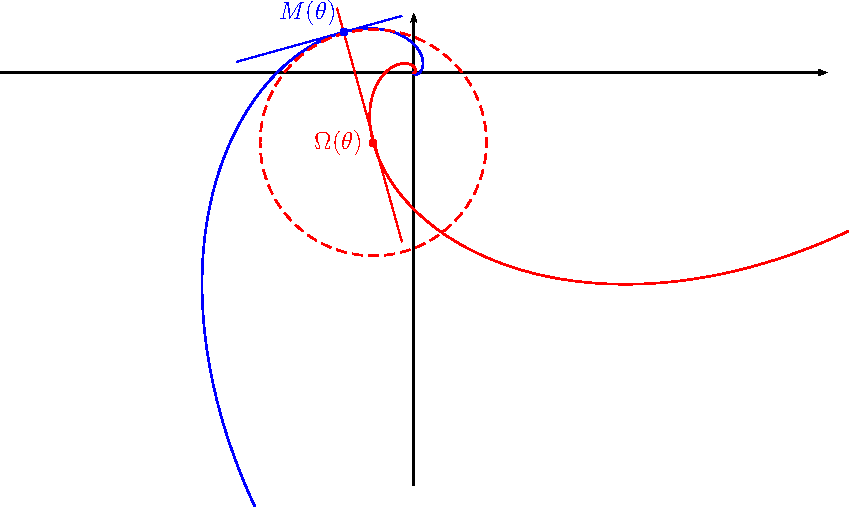
\includegraphics{../images/pdf/Du9L-1.pdf}$$
}
}
